
%%%%%%%%%%%%%%%%%%%%%%% file typeinst.tex %%%%%%%%%%%%%%%%%%%%%%%%%
%
% This is the LaTeX source for the instructions to authors using
% the LaTeX document class 'llncs.cls' for contributions to
% the Lecture Notes in Computer Sciences series.
% http://www.springer.com/lncs       Springer Heidelberg 2006/05/04
%
% It may be used as a template for your own input - copy it
% to a new file with a new name and use it as the basis
% for your article.
%
% NB: the document class 'llncs' has its own and detailed documentation,  see
% ftp://ftp.springer.de/data/pubftp/pub/tex/latex/llncs/latex2e/llncsdoc.pdf
%
%%%%%%%%%%%%%%%%%%%%%%%%%%%%%%%%%%%%%%%%%%%%%%%%%%%%%%%%%%%%%%%%%%%


\documentclass[runningheads, a4paper]{llncs}

\usepackage{xcolor} % Colors

\usepackage{tikz}
\usepackage{keyval}
\usepackage{pgfplots} % Bar charts

\usepgfplotslibrary{groupplots}

%\usepackage{groupplots}
%\usepgfplotslibrary{groupplots}
\pgfplotsset{compat=newest}
   
   
%
% Define bar chart colors
%
\definecolor{bblue}{HTML}{4F81BD}
\definecolor{rred}{HTML}{C0504D}
\definecolor{ggreen}{HTML}{9BBB59}
\definecolor{ppurple}{HTML}{9F4C7C}


\usepackage{amssymb}
\setcounter{tocdepth}{3}
\usepackage{graphicx}

\newcommand{\keywords}[1]{\par\addvspace\baselineskip
\noindent\keywordname\enspace\ignorespaces#1}







%%%%%%%%%%%%%%%%%%%%%%%%%%%%%%%%%%%%%%%%%
%           START OF COMMANDS
%%%%%%%%%%%%%%%%%%%%%%%%%%%%%%%%%%%%%%%%%


%%%%%%%%%%%%%%%%%%%%%%%%%%%%%%%%%
% Save results to be later used in addBarPlotResults
% #1: Train Small
% #2: Train Big
% #3: Train All
% #4: Test
%%%%%%%%%%%%%%%%%%%%%%%%%%%%%%%%%
\newcommand{\saveResultsFirst}[4]{
    \def\TrainSmallFirst{#1}%
    \def\TrainBigFirst{#2}%
    \def\TrainAllFirst{#3}%
    \def\TestFirst{#4}%
}

%%%%%%%%%%%%%%%%%%%%%%%%%%%%%%%%%
% Save results to be later used in addBarPlotResults
% #1: Train Small
% #2: Train Big
% #3: Train All
% #4: Test
%%%%%%%%%%%%%%%%%%%%%%%%%%%%%%%%%
\newcommand{\saveResultsSecond}[4]{
    \def\TrainSmallSecond{#1}%
    \def\TrainBigSecond{#2}%
    \def\TrainAllSecond{#3}%
    \def\TestSecond{#4}%
}

%%%%%%%%%%%%%%%%%%%%%%%%%%%%%%%%%
% Adds Results to Bars labeled by #1, #2
%
% Label #1 is used for saveResultsFirst
% Label #2 is used for saveResultsSecond
%
%%%%%%%%%%%%%%%%%%%%%%%%%%%%%%%%%
\newcommand{\addBarPlotResults}[2]{
    % TRAINING |w| < C    
    \addplot[style={bblue, fill=bblue, mark=none}]
    coordinates 
    {
        (#1,  \TrainSmallFirst)
        (#2,  \TrainSmallSecond)
    };
    
    % TRAINING |w| > C
    \addplot[style={rred, fill=rred, mark=none}]
    coordinates 
    {
        (#1,  \TrainBigFirst)
        (#2,  \TrainBigSecond)
    };
    
    % TRAINING ALL
    \addplot[style={ggreen, fill=ggreen, mark=none}]
    coordinates 
    {
        (#1,  \TrainAllFirst)
        (#2,  \TrainAllSecond)
    };
    
    % TESTING
    \addplot[style={ppurple, fill=ppurple, mark=none}]
    coordinates 
    {
        (#1,  \TestFirst)
        (#2,  \TestSecond)
    };
}



%%%%%%%%%%%%%%%%%%%%%%%%%%%%%%%%%
% Adds needed style to pgfplot
%%%%%%%%%%%%%%%%%%%%%%%%%%%%%%%%%
    \newcommand{\setPlotStyle}[0]{
        \pgfplotsset{xticklabel style={text width=2em, align=center}}
    }

%%%%%%%%%%%%%%%%%%%%%%%%%%%%%%%%%
% Starts groupplot with given style
%%%%%%%%%%%%%%%%%%%%%%%%%%%%%%%%%
    \newcommand{\beginGroupPlot}[0]{
    \begin{groupplot}[
        group style={group size= 2 by 2,  vertical sep=50pt},
        %        height = 4.5gcm, 
        ybar=4*\pgflinewidth, 
        ymin=0, 
        ymax=1,
        width  = 0.37*\textwidth, 
        enlarge x limits={abs=0.85cm}, 
        major x tick style = transparent, 
        ymajorgrids = true, 
        symbolic x coords={
            C=4,
            C=4 Q=3,
            C=4 Q=4,
            C=4 Q=5,
            C=4 Q=6,
            C=4 Q=7,
            C=4 Q=8,
            C=4 Q=9,
            C=4 Q=10,
            C=4 Q=11,
            C=4 Q=12,
            C=4 Q=13,
            C=4 Q=14,
            C=4 Q=15,
            C=5,
            C=5 Q=3,
            C=5 Q=4,
            C=5 Q=5,
            C=5 Q=6,
            C=5 Q=7,
            C=5 Q=8,
            C=5 Q=9,
            C=5 Q=10,
            C=5 Q=11,
            C=5 Q=12,
            C=5 Q=13,
            C=5 Q=14,
            C=5 Q=15
        },
        xtick = data, 
        scaled y ticks = false, 
        legend cell align=right, 
        legend columns=-1
        legend style={
            at={(-0.76, -0.7)}, 
            anchor=south east,
            column sep=15ex
        }
        ]
    }%beginGroupPlot
    
%%%%%%%%%%%%%%%%%%%%%%%%%%%%%%%%%
% Sets legends for Bar plot
%%%%%%%%%%%%%%%%%%%%%%%%%%%%%%%%%
    \newcommand{\setPlotLegend}[0]{
        \legend{Training $|w|<C$,  Training $|w|>C$,  Training All,  Testing}
    }
    
%%%%%%%%%%%%%%%%%%%%%%%%%%%%%%%%%%%%%%%%%
%           END OF COMMANDS
%%%%%%%%%%%%%%%%%%%%%%%%%%%%%%%%%%%%%%%%%




\begin{document}

\mainmatter  % start of an individual contribution

\title{A Stochastic Approach to Optimization of Deterministic Finite Automata}

% a short form should be given in case it is too long for the running head
\titlerunning{Algorithms and Computability}

\author{Jakub Ciecierski \and Bartlomiej Dybisz \\ 
\textit{Warsaw University of Technology, \\
Faculty of Mathematics and Information Science.}}
%
\authorrunning{Algorithms and Computability}

\toctitle{Algorithms and Computability}
\tocauthor{Methodology}
\maketitle

\section{Modeling}

\begin{figure}[h]
\label{fig:class_automata}
\caption{Class diagram of Automata module}
    \includegraphics[width=0.85\textwidth]{res/uml/classes/automata.jpg}
\end{figure}

\begin{figure}[h]
\label{fig:class_opt_main}
\caption{Class diagram of Optimization module }
    \includegraphics[width=0.85\textwidth]{res/uml/classes/optimizationMain.jpg}
\end{figure}


\begin{figure}[h]
\label{fig:class_opt_alg}
\caption{Class diagram of Optimization Algorithm module}
    \includegraphics[width=0.85\textwidth]{res/uml/classes/optimizationAlg.jpg}
\end{figure}

\begin{figure}[h]
\label{fig:state_opt}
\caption{State diagram of Optimization}
    \includegraphics[width=0.85\textwidth]{res/uml/states/optimizer.jpg}
\end{figure}

\begin{figure}[h]
\label{fig:state_pso}
\caption{State diagram of PSO}
    \includegraphics[width=0.85\textwidth]{res/uml/states/pso.jpg}
\end{figure}



\section{Experiments}

\subsection{Reconstruction}
\subsection{Approximation}

\section{Results}


%--------------------------------------------------------------------------------------
%--------------------------------------------------------------------------------------
\subsection{Reconstruction}



%--------------------------------------------------------------------------------------
%--------------------------------------------------------------------------------------




%%%%%%%%%%%%%%%%%%%%%%%%%%%%%%%%%%%%%
% GROUP BAR PLOT
% RECON     {C4, C5}
% CLASSES   {4, 6, 10, 15.}
% DFA ID    [1, 5]
%%%%%%%%%%%%%%%%%%%%%%%%%%%%%%%%%%%%%

\begin{figure}[h]
\caption{Reconstruction. Five Automata Classes 4, 6, 10, 15}



\setPlotStyle
\hspace{-3.2cm}
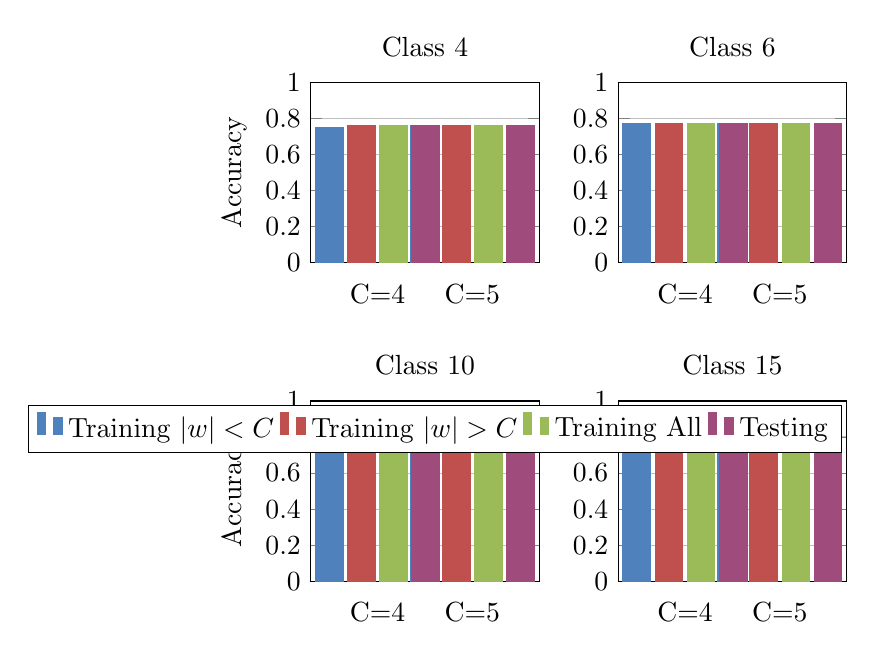
\begin{tikzpicture}

%%%%%%%%%%%%%%%%%%%%
% GROUPPLOT
%%%%%%%%%%%%%%%%%%%%

\beginGroupPlot
    

%%%%%%%%%%%%%%%%%%%%
% DFA ID:  1
%%%%%%%%%%%%%%%%%%%%
    \nextgroupplot[title=Class 4,  ylabel=Accuracy]%
    \saveResultsFirst   {0.75}{0.76}{0.76}{0.76}
    \saveResultsSecond  {0.76}{0.76}{0.76}{0.76}
    \addBarPlotResults  {C=4}{C=5}
    
    \nextgroupplot[title=Class 6]%
    \saveResultsFirst   {0.77}{0.77}{0.77}{0.77}
    \saveResultsSecond  {0.77} {0.77}{0.77}{0.77}
    \addBarPlotResults  {C=4}{C=5}
    
    \nextgroupplot[title=Class 10, ylabel=Accuracy]
    \saveResultsFirst   {0.83}{0.83}{0.83}{0.83}
    \saveResultsSecond  {0.83}{0.83}{0.83}{0.83}
    \addBarPlotResults  {C=4}{C=5}
    
    
    \nextgroupplot[title=Class 15]%TODO
    \saveResultsFirst   {0.86}{0.86}{0.86}{0.86}
    \saveResultsSecond  {0.86}{0.86}{0.86}{0.86}
    \addBarPlotResults  {C=4}{C=5}
        

%%%%%%%%%%%%%%%%%%%%
% LEGEND
%%%%%%%%%%%%%%%%%%%%

\setPlotLegend


\end{groupplot}
    
\end{tikzpicture}
    

\end{figure}







\begin{figure}[h]
    \caption{Reconstruction. Example of Testing Set Quality across the PSO interval One Automaton $A(4.1)$}

%%%%%%%%%%%%%%%%%%%%%%%%%%%%%%%%%%%%%
% GROUP LINE PLOT
% RECON     {C4, C5}
% CLASSES   {4, 6, 10, 15.}
% DFA ID    {0}
%%%%%%%%%%%%%%%%%%%%%%%%%%%%%%%%%%%%%

\setPlotStyle
\hspace{-2.5cm}
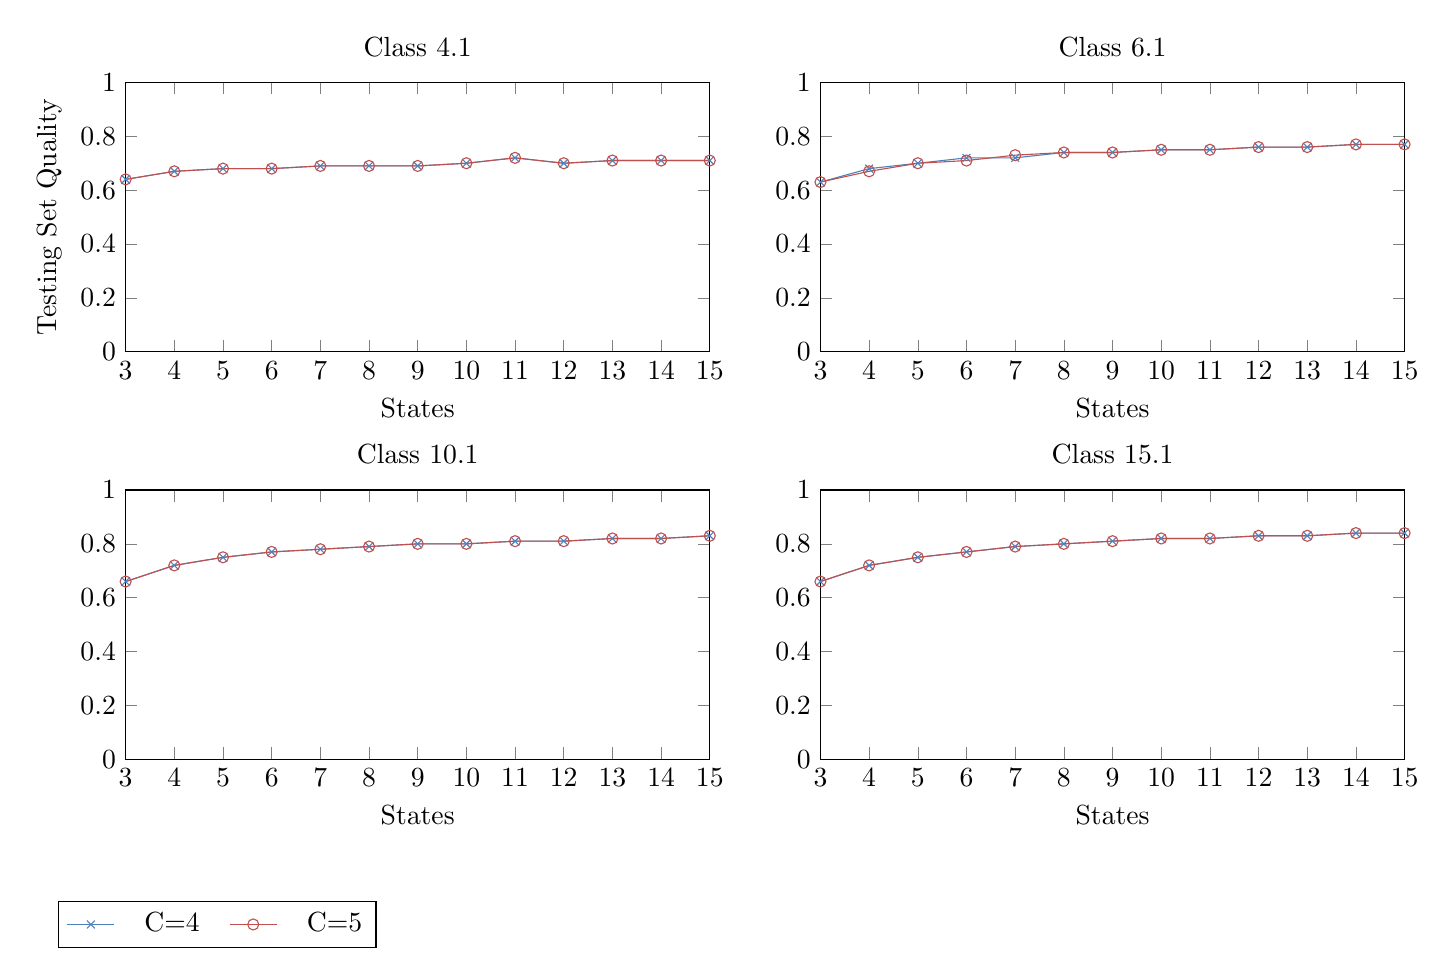
\begin{tikzpicture}

\begin{groupplot}[group style={group size= 2 by 2,
        vertical sep=50pt, horizontal sep=40pt}, 
        height=5cm,
        width=9cm,
        xtick={3,4,5,6,7,8,9,10,11,12,13,14,15},
        xlabel=States,
        ymax=1.0, 
        ymin=0.0, 
        xmin=3,
        xmax=15,  
        legend cell align=left, 
        legend columns=-1, 
        legend style={
            at={(-0.76, -0.7)}, 
            anchor=south east, 
            column sep=2ex
        }
       ]


%%%%%%%%%%%%%%%%%%%%
% CLASS     4
% DFA ID    1
%%%%%%%%%%%%%%%%%%%%

\nextgroupplot[title=Class 4.1,  ylabel=Testing Set Quality]

% RECONS_C4_CL4_1
\addplot[color=bblue, mark=x] coordinates {
    (3, 0.64)
    (4, 0.67)
    (5, 0.68)
    (6, 0.68)
    (7, 0.69)
    (8, 0.69)
    (9, 0.69)
    (10, 0.70)
    (11, 0.72)
    (12, 0.70)
    (13, 0.71)
    (14, 0.71)
    (15, 0.71)
};


% RECONS_C5_CL4_1
\addplot[color=rred, mark=o] coordinates {
    (3, 0.64)
    (4, 0.67)
    (5, 0.68)
    (6, 0.68)
    (7, 0.69)
    (8, 0.69)
    (9, 0.69)
    (10, 0.70)
    (11, 0.72)
    (12, 0.70)
    (13, 0.71)
    (14, 0.71)
    (15, 0.71)
};


%%%%%%%%%%%%%%%%%%%%
% CLASS     6
% DFA ID    1
%%%%%%%%%%%%%%%%%%%%
\nextgroupplot[title=Class 6.1]
% RECONS_C4_CL6_1
\addplot[color=bblue, mark=x] coordinates {
    (3, 0.63)
    (4, 0.68)
    (5, 0.70)
    (6, 0.72)
    (7, 0.72)
    (8, 0.74)
    (9, 0.74)
    (10, 0.75)
    (11, 0.75)
    (12, 0.76)
    (13, 0.76)
    (14, 0.77)
    (15, 0.77)
};


% RECONS_C5_CL6_1
\addplot[color=rred, mark=o] coordinates {
    (3, 0.63)
    (4, 0.67)
    (5, 0.70)
    (6, 0.71)
    (7, 0.73)
    (8, 0.74)
    (9, 0.74)
    (10, 0.75)
    (11, 0.75)
    (12, 0.76)
    (13, 0.76)
    (14, 0.77)
    (15, 0.77)
};


%%%%%%%%%%%%%%%%%%%%
% CLASS     10
% DFA ID    1
%%%%%%%%%%%%%%%%%%%%
\nextgroupplot[title=Class 10.1]

% RECONS_C4_CL10_1
\addplot[color=bblue, mark=x] coordinates {
    (3, 0.66)
    (4, 0.72)
    (5, 0.75)
    (6, 0.77)
    (7, 0.78)
    (8, 0.79)
    (9, 0.80)
    (10, 0.80)
    (11, 0.81)
    (12, 0.81)
    (13, 0.82)
    (14, 0.82)
    (15, 0.83)
};

% RECONS_C5_CL10_1
\addplot[color=rred, mark=o] coordinates {
    (3, 0.66)
    (4, 0.72)
    (5, 0.75)
    (6, 0.77)
    (7, 0.78)
    (8, 0.79)
    (9, 0.80)
    (10, 0.80)
    (11, 0.81)
    (12, 0.81)
    (13, 0.82)
    (14, 0.82)
    (15, 0.83)
};


%%%%%%%%%%%%%%%%%%%%
% CLASS     15
% DFA ID    1
%%%%%%%%%%%%%%%%%%%%
\nextgroupplot[title=Class 15.1]

% RECONS_C4_CL15_1
\addplot[color=bblue, mark=x] coordinates {
    (3, 0.66)
    (4, 0.72)
    (5, 0.75)
    (6, 0.77)
    (7, 0.79)
    (8, 0.80)
    (9, 0.81)
    (10, 0.82)
    (11, 0.82)
    (12, 0.83)
    (13, 0.83)
    (14, 0.84)
    (15, 0.84)
};


% RECONS_C5_CL15_1
\addplot[color=rred, mark=o] coordinates {
    (3, 0.66)
    (4, 0.72)
    (5, 0.75)
    (6, 0.77)
    (7, 0.79)
    (8, 0.80)
    (9, 0.81)
    (10, 0.82)
    (11, 0.82)
    (12, 0.83)
    (13, 0.83)
    (14, 0.84)
    (15, 0.84)
};

\addlegendentry{C=4}
\addlegendentry{C=5}

\end{groupplot}
\end{tikzpicture}


\end{figure}




%--------------------------------------------------------------------------------------
%--------------------------------------------------------------------------------------
\subsection{Approximation}



\begin{figure}[h]
    \caption{Approximation. Automata [1,5]. Classes 20, 30, 50, 80}
    
%%%%%%%%%%%%%%%%%%%%%%%%%%%%%%%%%%%%%
% GROUP BAR PLOT
% APPROX    {C4, C5}
% CLASSES   {20, 30, 50, 80.}
% DFA ID    [1, 5]
%%%%%%%%%%%%%%%%%%%%%%%%%%%%%%%%%%%%%

\setPlotStyle
\hspace{-3.2cm}
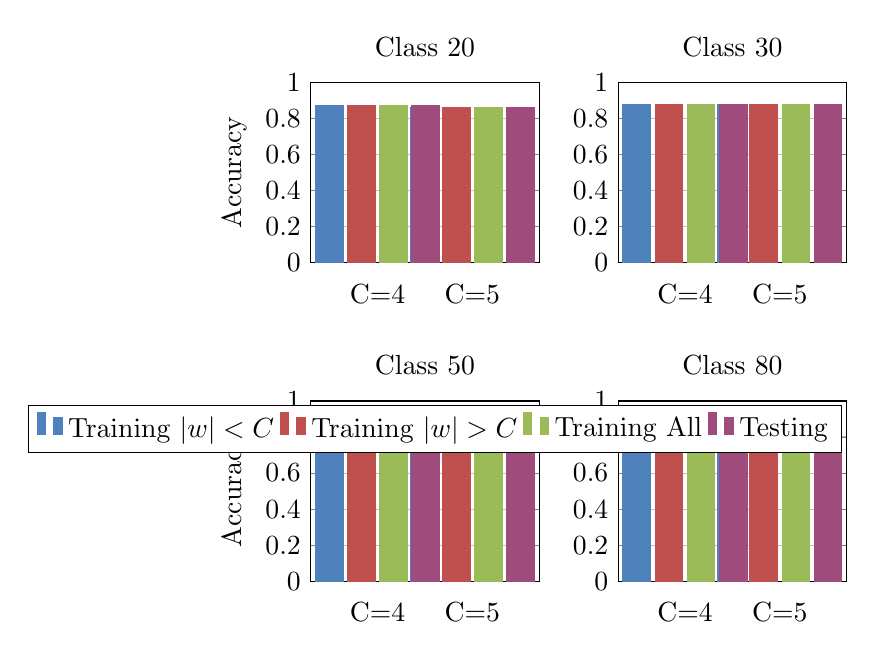
\begin{tikzpicture}

%%%%%%%%%%%%%%%%%%%%
% GROUPPLOT
%%%%%%%%%%%%%%%%%%%%

\beginGroupPlot

%%%%%%%%%%%%%%%%%%%%
% DFA ID:  1
%%%%%%%%%%%%%%%%%%%%

\nextgroupplot[title=Class 20, ylabel=Accuracy]
\saveResultsFirst   {0.87}{0.87}{0.87}{0.87}
\saveResultsSecond  {0.86}{0.86}{0.86}{0.86}
\addBarPlotResults  {C=4}{C=5}

\nextgroupplot[title=Class 30]
\saveResultsFirst   {0.88}{0.88}{0.88}{0.88}
\saveResultsSecond  {0.88}{0.88}{0.88}{0.88}
\addBarPlotResults  {C=4}{C=5}

\nextgroupplot[title=Class 50, ylabel=Accuracy]
\saveResultsFirst   {0.89}{0.89}{0.89}{0.89}
\saveResultsSecond  {0.89}{0.89}{0.89}{0.89}
\addBarPlotResults  {C=4}{C=5}

\nextgroupplot[title=Class 80]
\saveResultsFirst   {0.90}{0.90}{0.90}{0.90}
\saveResultsSecond  {0.90}{0.90}{0.90}{0.90}
\addBarPlotResults  {C=4}{C=5}


%%%%%%%%%%%%%%%%%%%%
% LEGEND
%%%%%%%%%%%%%%%%%%%%
\setPlotLegend

\end{groupplot}

\end{tikzpicture}

\end{figure}



\begin{figure}[h]
\caption{Approximation. Example of Testing quality across the PSO interval. Classes 20, 30, 50, 80}
%%%%%%%%%%%%%%%%%%%%%%%%%%%%%%%%%%%%%
% GROUP LINE PLOT
% APPROX    {C4, C5}
% CLASSES   {20, 30, 50, 80.}
% DFA ID    {0}
% STATES    {4,6,8,10,12}
%%%%%%%%%%%%%%%%%%%%%%%%%%%%%%%%%%%%%

\setPlotStyle
\hspace{-2.0cm}
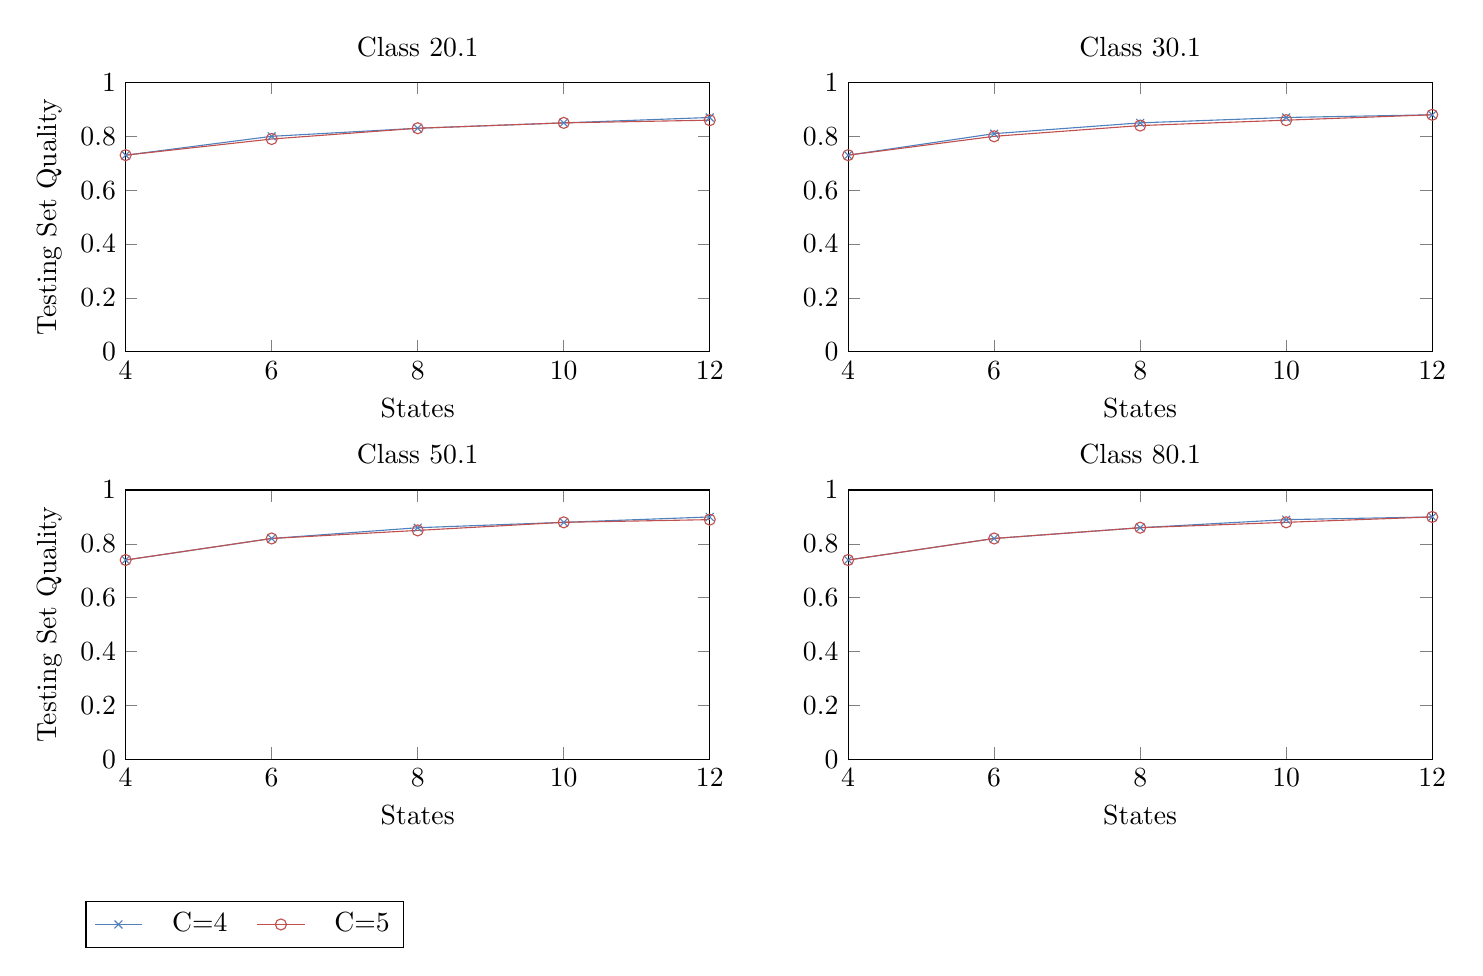
\begin{tikzpicture}



\begin{groupplot}[group style={group size= 2 by 2,  
        vertical sep=50pt, horizontal sep=50pt},
    xtick={4,6,8,10,12},
    height=5cm,
    width=9cm,
    xlabel=States, 
    ymax=1.0, 
    ymin=0.0, 
    xmin=4, 
    xmax=12,   
    legend cell align=left, 
    legend columns=-1, 
    legend style={
       	at={(-0.76, -0.7)}, 
       	anchor=south east, 
       	column sep=2ex
    }]



%%%%%%%%%%%%%%%%%%%%
% CLASS     20
% DFA ID    1
%%%%%%%%%%%%%%%%%%%%

\nextgroupplot[title=Class 20.1,  ylabel=Testing Set Quality]
% APPROX_C4_CL20_1
\addplot[color=bblue, mark=x] coordinates {
	(4, 0.73)
	(6, 0.80)
	(8, 0.83)
	(10, 0.85)
	(12, 0.87)
};


% APPROX_C5_CL20_1
\addplot[color=rred, mark=o] coordinates {
    (4, 0.73)
    (6, 0.79)
    (8, 0.83)
    (10, 0.85)
    (12, 0.86)
};



%%%%%%%%%%%%%%%%%%%%
% CLASS     30
% DFA ID    1
%%%%%%%%%%%%%%%%%%%%

\nextgroupplot[title=Class 30.1]
% APPROX_C4_CL30_1
\addplot[color=bblue, mark=x] coordinates {
	(4, 0.73)
	(6, 0.81)
	(8, 0.85)
	(10, 0.87)
	(12, 0.88)
};

% APPROX_C5_CL30_1
\addplot[color=rred, mark=o] coordinates {
	(4, 0.73)
	(6, 0.80)
	(8, 0.84)
	(10, 0.86)
	(12, 0.88)
};





%%%%%%%%%%%%%%%%%%%%
% CLASS     50
% DFA ID    1
%%%%%%%%%%%%%%%%%%%%
\nextgroupplot[title=Class 50.1, ylabel=Testing Set Quality]
% APPROX_C4_CL50_1
\addplot[color=bblue, mark=x] coordinates {
	(4, 0.74)
	(6, 0.82)
	(8, 0.86)
	(10, 0.88)
	(12, 0.90)
};

    % APPROX_C5_CL50_1
    \addplot[color=rred, mark=o] coordinates {
        (4, 0.74)
        (6, 0.82)
        (8, 0.85)
        (10, 0.88)
        (12, 0.89)
};



%%%%%%%%%%%%%%%%%%%%
% CLASS     80
% DFA ID    1
%%%%%%%%%%%%%%%%%%%%

\nextgroupplot[title=Class 80.1]
% APPROX_C4_CL80_1
\addplot[color=bblue, mark=x] coordinates {
	(4, 0.74)
	(6, 0.82)
	(8, 0.86)
	(10, 0.89)
	(12, 0.90)
};
\addlegendentry{C=4}

% APPROX_C5_CL80_1
\addplot[color=rred, mark=o] coordinates {
	(4, 0.74)
	(6, 0.82)
	(8, 0.86)
	(10, 0.88)
	(12, 0.90)
};
\addlegendentry{C=5}

\end{groupplot}
\end{tikzpicture}


\end{figure}





















\begin{thebibliography}{4}

%\bibitem

\end{thebibliography}

\end{document}
